\section{Einführung in die Programmierung}

\begin{frame}{Erwartungen und Vorkenntnisse}
    \begin{itemize}
        \item Erwartungen an den Kurs?
        \item Bereits Programmierkenntnisse aus Schule/Universität?
        \item Kursziele 
            \begin{itemize}
                \item grundlegendes Verständnis
                \item ``mit Informatikern reden können"
                \item Angst nehmen
            \end{itemize}
    \end{itemize}
\end{frame}

\begin{frame}{Die Programmiersprache Python}
\begin{columns}
    \column{0.5\textwidth}
    \begin{itemize}
        \item Cool
    \end{itemize}
    \column{0.5\textwidth}
    \centering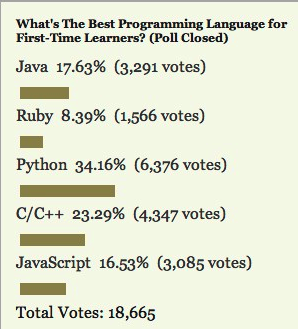
\includegraphics[scale=0.5]{images/best_lang} 
\end{columns}
\end{frame}

